% \pagenumbering{arabic}

\Large
\label{Chapter_4}

The STRATA framework secures resource-constrained industrial devices by partitioning trust across tiered layers, so that speed, verifiability, and cost are each served where they are cheapest to obtain rather than traded against one another on a single ledger. Its construction proceeds through four elements: (a) a behavioural trust-scoring stratum that scores device conduct in real time on a fast permissioned layer, (b) a consensus and coordination stratum that finalises validated behaviour under permissioned consensus, (c) a public anchoring stratum that commits compact proofs to an open layer for external audit, and (d) two cross-cutting planes that carry quantum-resilient identity, revocation, and post-quantum protection across all three strata. This chapter details the design and operational logic of each element, the resource-aware placement principle that binds them, and the two ledger substrates on which the framework is realised. Figure~\ref{fig:strata-arch} presents the overall architecture, with the three strata separated by the trust-partition boundary and the two planes spanning them.


\begin{figure}[t]
  \centering
  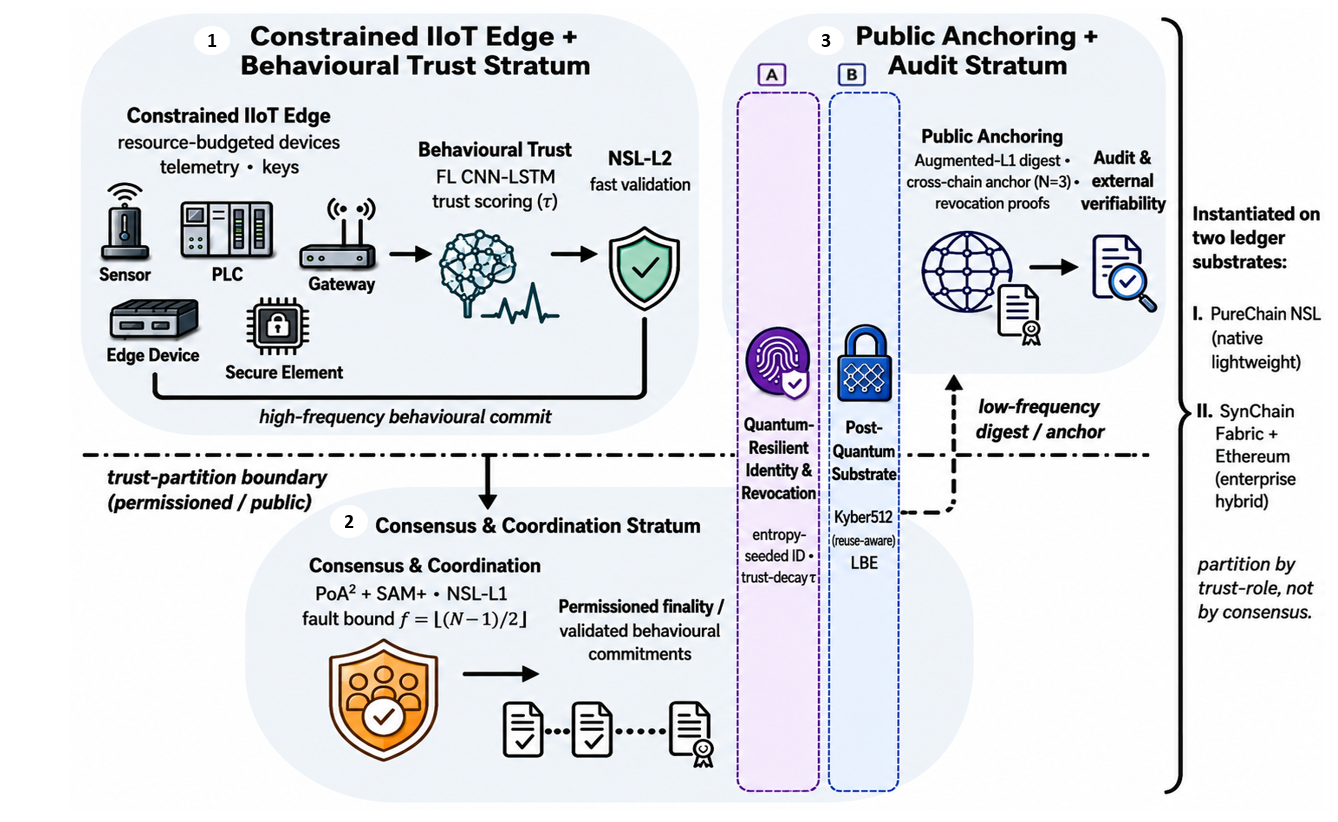
\includegraphics[width=\textwidth]{figures/Picture133.PNG}
 \caption[STRATA framework architecture]{Architecture of the proposed STRATA
framework. The solid arrow marks the high-frequency behavioural commitment
retained inside the permissioned domain, and the dashed arrow the
low-frequency digest that crosses the trust-partition boundary to the public
anchor. Planes~A and~B span all three strata, and the tiered core is realised
on two ledger substrates, PureChain NSL and SynChain Fabric+Ethereum,
partitioning by trust-role rather than by consensus mechanism.}
  \label{fig:strata-arch}
\end{figure}

The objective of STRATA is the greatest attainable trustworthy security that a constrained deployment can sustain, obtained by assigning each security operation to the stratum whose trust characteristics match it. Let $\sigma$ denote such an assignment of operations to strata, $\mathcal{T}(\sigma)$ the trustworthiness it delivers, and $\mathcal{R}(\sigma)$ its resource footprint. The design solves

\begin{equation}
\label{eq:strata-objective}
\sigma^{\star} \;=\; \arg\max_{\sigma}\; \mathcal{T}(\sigma)
\quad \text{subject to} \quad
\mathcal{R}_{\text{edge}}(\sigma) \le \mathcal{B}_{\text{edge}},
\;\;
\mathcal{R}_{\text{chain}}(\sigma) \le \mathcal{B}_{\text{chain}},
\end{equation}

where $\mathcal{B}_{\text{edge}}$ is the compute, memory, and energy budget of the constrained edge and $\mathcal{B}_{\text{chain}}$ the throughput and storage budget of the ledger. Trustworthiness combines behavioural detection fidelity with anchored verifiability,

\begin{equation}
\label{eq:strata-trust}
\mathcal{T}(\sigma) \;=\; \sum_{i=1}^{n} \big[\, w_{s}\, s_i \;+\; w_{\upsilon}\, \upsilon_i(\sigma) \,\big],
\end{equation}

in which $s_i \in [0,1]$ is the accumulated behavioural trust score of device $d_i$ (Section~\ref{sec:plane-a}), $\upsilon_i(\sigma)\in\{0,1\}$ indicates whether that device's security-relevant events are anchored and hence externally verifiable, and $w_{s}, w_{\upsilon}$ weight detection against verifiability. Equation~\eqref{eq:strata-objective} states the problem the strata jointly solve: the permissioned strata raise $s_i$ within the edge budget while the anchoring stratum raises $\upsilon_i$ within the ledger budget, so that neither term improves by exhausting the resources of the other. A centralised or single-ledger arrangement, by contrast, must satisfy both budgets on one layer and therefore cannot maximise either without violating the constraint that constrained hardware imposes.



\section{The Trust-Partitioning Principle and System Model}
\label{sec:strata-principle}

Security, speed, and scalability compete on any ledger placed on constrained industrial hardware, and no single-ledger design reconciles all three within a real device budget. STRATA resolves the tension by reassignment rather than compromise: each security responsibility is placed on the layer whose trust characteristics match it, so operations demanding speed run where consensus is cheap and operations demanding public accountability run where verification is open. This converts the trilemma from a balance to be struck into a placement to be solved, and it is the principle from which the rest of the framework follows.

The placement rests on a single observation. Security-relevant operations differ not only in what they protect but in the trust profile they require. A behavioural trust update issued many times per second needs deterministic, low-cost validation and tolerates a closed validator set. An identity revocation or an audit commitment occurs rarely, carries high value, and must be verifiable by parties outside the operating consortium. Treating both alike forces one ledger to be fast and public at once, which constrained budgets do not permit. Partitioning treats them differently by design.

\begin{definition}[Trust-partitioning]
\label{def:trust-partition}
A security architecture is trust-partitioned if every security-relevant operation $e$ is assigned to exactly one stratum according to its trust-role $\kappa(e)=(\phi_e,\nu_e,\xi_e)$, where $\phi_e$ is the operation's frequency, $\nu_e$ its value, and $\xi_e$ its required verifiability scope, such that high-frequency, low-value operations with consortium-internal verifiability are confined to a fast permissioned stratum, low-frequency, high-value operations with external verifiability are committed to a public anchoring stratum, and a single well-defined interface transfers state between the two.
\end{definition}

The partition is drawn by trust-role, not by consensus mechanism. This distinction carries the framework's generality: the same assignment of operations to strata can be realised on substrates whose consensus protocols differ entirely, a property developed in Section~\ref{sec:strata-substrates}.

\subsection{System Model}
\label{subsec:strata-sysmodel}

The framework serves a set $\mathcal{D}=\{d_1,\dots,d_n\}$ of resource-constrained industrial devices, each generating telemetry and holding key material at the constrained edge. Above this base, security responsibility divides across three strata and two cross-cutting planes.

The behavioural trust stratum scores device conduct in real time. A lightweight federated CNN--LSTM intrusion-detection engine evaluates network and metadata behaviour and emits a per-window trust score $q_i \in [0,1]$, committed at device rate on the fast permissioned layer (NSL-L2) so that the verdict is recorded rather than left on the host that computed it. The full detection design is given in Section~\ref{sec:strata-trust}.

The consensus and coordination stratum finalises those commitments. Permissioned finalisation uses the Proof-of-Authority-and-Association protocol with the Smart Auto-Mining Plus mechanism on the coordination layer (NSL-L1), tolerating up to $f=\lfloor (N-1)/2 \rfloor$ faulty or unavailable validators for $N$ authorities. Deterministic finality bounds the latency of a behavioural decision without exposing it publicly.

The public anchoring stratum carries only what external accountability requires. Compact digests of finalised state and revocation proofs cross the trust-partition boundary and are committed to an open layer (Augmented-L1), cross-chain-anchored to a public chain where interoperability demands it. Payloads never cross; only proofs do, which preserves confidentiality while enabling open verification. The anchoring design appears in Section~\ref{sec:strata-anchor}.

Two planes span the strata rather than residing in any one. The identity and revocation plane, detailed in Section~\ref{sec:strata-identity}, binds each device to an entropy-seeded identity and governs revocation by a trust-decay law, so a verdict raised in the trust stratum propagates to a revocation proof anchored in the public stratum. The post-quantum plane protects credentials and anchored records with lattice-based primitives against both classical and quantum adversaries. Figure~\ref{fig:strata-arch} places both planes as vertical elements to indicate this span.

\subsection{Verifiability Under Partitioning}
\label{subsec:strata-theorem}

A partition is sound only if confining an operation to the permissioned side preserves its public verifiability. The following establishes that partitioning meets this condition.

\begin{theorem}[Verifiability preservation]
\label{thm:verifiability}
Let a security-relevant event $e$ be finalised within the permissioned strata, and let its digest $H(e)$ be anchored on the public stratum under an immutable ledger, where $H$ is collision-resistant. Then any party with access to the public stratum alone can verify the integrity of $e$, and the partition introduces no loss of verifiability relative to committing $e$ in full on the public stratum.
\end{theorem}

\begin{proof}[Proof sketch]
Verifying $e$ means confirming that the copy presented to a verifier is the one finalised. A verifier recomputes $H(e')$ from a presented $e'$ and compares it to the anchored $H(e)$; equality holds if and only if $e'=e$, except with negligible probability under collision resistance. Immutability of the public stratum guarantees the anchored value cannot be altered after commitment, so the reference is trustworthy. Integrity of $e$ is therefore verifiable from the public stratum without access to the permissioned strata. Committing $e$ publicly in full would expose the same guarantee through $e$ itself; the partition transfers only the proof $H(e)$ to the public stratum and confines the payload, so no verifiability is lost.
\end{proof}

Theorem~\ref{thm:verifiability} is the formal counterpart of the placement argument. Because the proof of integrity, not the payload, is what public accountability requires, the high-value proof is anchored publicly while the high-frequency payload stays permissioned, which is the separation Definition~\ref{def:trust-partition} prescribes. Table~\ref{tab:strata-map} sets each element of the framework against the review gap it closes and the research question it answers, so the architecture reads as a principled response to the gaps established earlier rather than a set of untested mechanisms.


\begin{table}[t]
  \centering
  \footnotesize
  \setlength{\tabcolsep}{5pt}
  \renewcommand{\arraystretch}{1.3}
  \caption{Mapping of each STRATA stratum and plane to its function, the review gap it closes, and the research question it addresses.}
  \label{tab:strata-map}
  \begin{tabularx}{\textwidth}{@{}
      >{\raggedright\arraybackslash}p{3.0cm}
      >{\raggedright\arraybackslash}X
      >{\raggedright\arraybackslash}p{2.4cm}
      >{\raggedright\arraybackslash}p{0.9cm}@{}}
    \toprule
    \textbf{Element} & \textbf{Function} & \textbf{Gap closed} & \textbf{RQ} \\
    \midrule
    Stratum~1 \newline Behavioural Trust
      & Federated CNN--LSTM behavioural trust scoring on the fast permissioned layer
      & Mutable verdict & RQ2 \\
    Stratum~2 \newline Consensus \& Coordination
      & Permissioned finalisation via PoA$^2$ and SAM+; fault bound $f=\lfloor(N{-}1)/2\rfloor$
      & Placement (speed) & RQ1 \\
    Stratum~3 \newline Public Anchoring
      & Digest anchoring and cross-chain commitment of proofs
      & Placement (public) & RQ1 \\
    Plane~A \newline Identity \& Revocation
      & Entropy-seeded identity and trust-decay revocation across strata
      & Accountability & RQ5 \\
    Plane~B \newline Post-Quantum Substrate
      & Compressed Kyber512 and lattice-based encryption for credentials and anchors
      & Quantum durability & RQ3 \\
    \addlinespace
    Dual-substrate realisation
      & Same partition on PureChain NSL and on SynChain Fabric+Ethereum
      & Substrate dependence & RQ4 \\
    \bottomrule
  \end{tabularx}
\end{table}

The strata and planes are specified individually in the sections that follow, beginning with the behavioural trust-scoring stratum. Table~\ref{tab:notation} collects the principal notation used throughout the chapter.

\begin{table}[htbp]
  \centering
  \footnotesize
  \setlength{\tabcolsep}{5pt}
  \renewcommand{\arraystretch}{1.25}
  \caption{Principal notation used in the specification of STRATA.}
  \label{tab:notation}
  \begin{tabularx}{\textwidth}{@{}
      >{\raggedright\arraybackslash}p{2.2cm}
      >{\raggedright\arraybackslash}X
      >{\raggedright\arraybackslash}p{2.6cm}@{}}
    \toprule
    \textbf{Symbol} & \textbf{Meaning} & \textbf{Introduced in} \\
    \midrule
    $\mathcal{D}$, $d_i$ & Set of constrained devices; device $i$ & Section~\ref{subsec:strata-sysmodel} \\
    $\sigma$ & Assignment of security operations to strata & Eq.~\eqref{eq:strata-objective} \\
    $\kappa(e)$ & Trust-role of operation $e$: frequency, value, verifiability scope & Definition~\ref{def:trust-partition} \\
    $q_i$ & Per-window behavioural trust score produced by Stratum~1 & Eq.~\eqref{eq:strata-flag} \\
    $\delta$ & Flag threshold applied to $q_i$ & Eq.~\eqref{eq:strata-flag} \\
    $s_i(t)$ & Accumulated device trust score maintained by Plane~A & Eq.~\eqref{eq:trust-decay} \\
    $\beta$ & Retention factor of the trust-decay law & Eq.~\eqref{eq:trust-decay} \\
    $\tau$ & Revocation threshold applied to $s_i(t)$ & Section~\ref{sec:plane-a} \\
    $S_i(t)$, $\mu_S$ & Anomaly streak counter; streak limit & Eq.~\eqref{eq:revoke-condition} \\
    $\omega_i$, $\theta$ & Validator authority weight; weighted acceptance threshold & Eq.~\eqref{eq:poa2-accept} \\
    $\rho_i(t)$, $\gamma$ & Validator reliability; reliability decay factor & Eq.~\eqref{eq:poa2-reliability} \\
    $N$, $f$ & Active validator count; tolerated faulty validators & Eq.~\eqref{eq:poa2-fault} \\
    $E$, $\lambda$ & Epoch span; verdict arrival rate & Definition~\ref{def:epoch} \\
    $R_k$, $\mathcal{C}_k$ & Epoch root; public commitment for epoch $k$ & Eqs.~\eqref{eq:merkle-root}, \eqref{eq:anchor-tuple} \\
    $\pi$ & Evidence bundle supporting a revocation & Eq.~\eqref{eq:revoke} \\
    $H(\cdot)$ & Collision-resistant hash function & Theorem~\ref{thm:verifiability} \\
    $c_{\mathrm{tx}}$, $\lambda_r$ & Fee per public commitment; revocation rate & Eq.~\eqref{eq:anchor-cost} \\
    \bottomrule
  \end{tabularx}
\end{table}

\section{The Behavioural Trust-Scoring Stratum}
\label{sec:strata-trust}
The behavioural trust-scoring stratum is where compromise is detected and turned into a committed verdict. Industrial attacks rarely match a fixed signature and usually surface only as a drift in how a device communicates, so detection here is learned from behaviour rather than matched against rules. The stratum runs a lightweight federated intrusion-detection engine at the constrained edge, scores each device's conduct as a continuous value, and writes that score to the fast permissioned layer, so the trust decision becomes a recorded fact rather than a transient computation on the device that produced it. The engine and its placement follow a lightweight federated design tailored to constrained industrial nodes.

Two requirements shape the engine. It must run inside the compute, memory, and energy budget of an industrial edge node, and it must produce a decision fast enough to gate high-frequency operation. A federated learning arrangement meets the first by keeping raw telemetry on the device and exchanging only model updates, and a deliberately trimmed network meets the second by keeping inference cheap. Figure~\ref{fig:strata-fl-arch} shows the arrangement: constrained clients train locally, a coordinator aggregates their updates into a global model, and the resulting trust scores are committed through the fast layer to the ledger.

\begin{figure}[t]
  \centering
  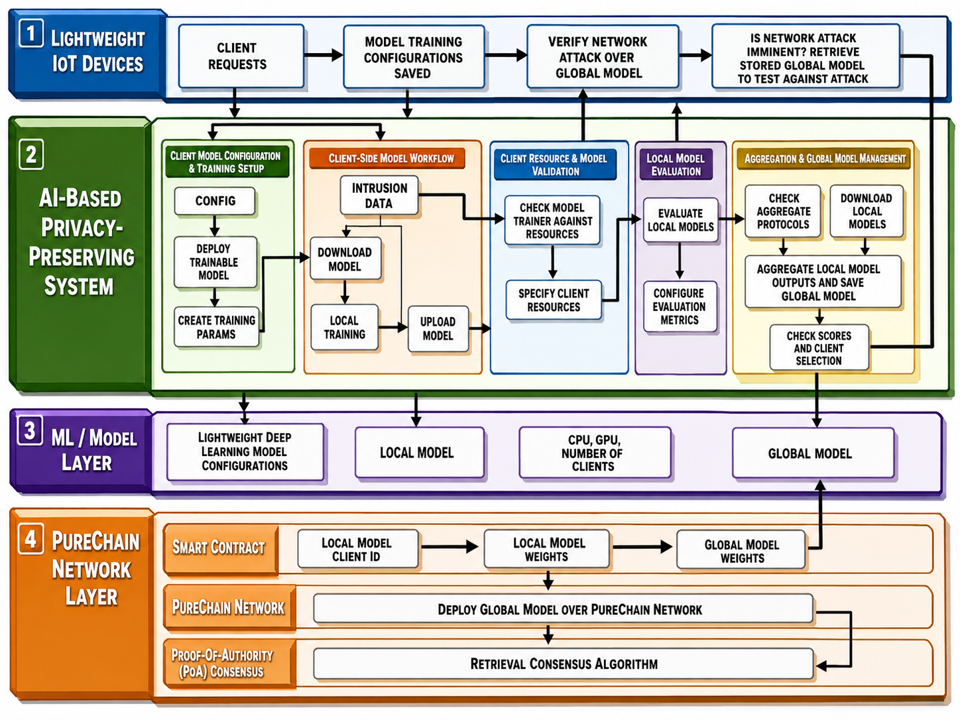
\includegraphics[width=\textwidth]{figures/Picture 16.png}
  \caption{Architecture of the behavioural trust-scoring stratum, recaptured from the published lightweight federated design~\cite{amadi2026lightweight}. Resource-constrained clients train a trimmed CNN--LSTM locally on their own telemetry; a coordinator aggregates the local updates into a global model by federated averaging; the resulting per-device trust scores are registered through the fast permissioned layer for commitment.}
  \label{fig:strata-fl-arch}
\end{figure}

\subsection{Detection Model}
\label{subsec:strata-model}
The engine pairs a one-dimensional convolutional front end with a recurrent stage. The convolutional layers act as a feature compressor over packet-flow statistics, capturing short-range structure such as burst rates and protocol flags, and the recurrent stage models the longer-range temporal dependence of an attack that unfolds across a session. A purely convolutional model captures local patterns but lacks temporal memory, while a standalone recurrent model is costlier on constrained hardware; the hybrid keeps inference light by letting the convolutional layers reduce dimensionality before the recurrent stage operates. The engine and its trust-threshold decision are shown in Figure~\ref{fig:strata-cnnlstm}: telemetry is compressed by the convolutional and pooling stage, the LSTM stage captures temporal dependence, and the softmax output yields the trust score $q_i$, which the threshold test $q_i < \delta$ turns into either a committed trust score on the fast permissioned layer or a revocation event raised to the identity plane.

\begin{figure}[t]
  \centering
  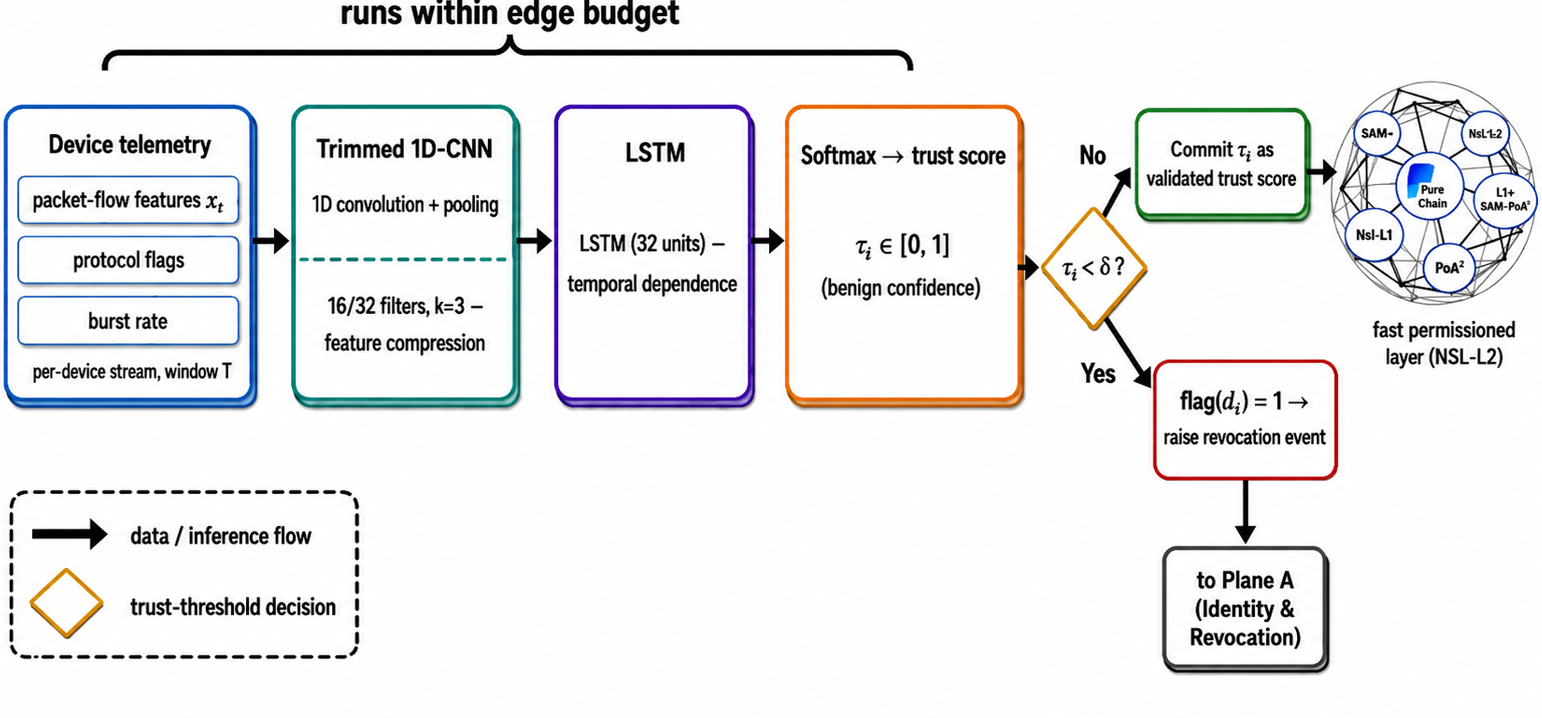
\includegraphics[width=\textwidth]{figures/Picture 15.PNG}
  \caption{Behavioural trust-scoring engine of Stratum~1. Device telemetry over a window $T$ passes through a trimmed one-dimensional CNN and pooling stage for feature compression, an LSTM stage for temporal dependence, and a softmax that yields the per-device trust score $q_i\in[0,1]$. The threshold test $q_i<\delta$ then either commits the score as a validated trust score to the fast permissioned layer or raises a revocation event to the identity plane.}
  \label{fig:strata-cnnlstm}
\end{figure}

For an input sequence $\mathbf{x} \in \mathbb{R}^{T \times d}$ of $d$-dimensional per-step feature vectors over a window of length $T$, the convolutional response of the $k$-th filter with kernel size $h$ is
\begin{equation}
\label{eq:strata-conv}
c_t^{(k)} \;=\; \mathrm{ReLU}\!\left( \sum_{i=0}^{h-1} \mathbf{w}_i^{(k)} \cdot \mathbf{x}_{t+i} + b^{(k)} \right),
\end{equation}
with same-length padding so boundary indices remain well defined. The pooled convolutional features pass to the LSTM stage, whose final hidden state $\mathbf{h}_T$ is mapped to a class distribution over the $C$ attack categories by
\begin{equation}
\label{eq:strata-softmax}
\hat{y}_j \;=\; \frac{\exp(z_j)}{\sum_{\ell=1}^{C} \exp(z_\ell)}, \qquad \mathbf{z} \;=\; \mathbf{W}_{\text{out}}\,\mathbf{h}_T + \mathbf{b}_{\text{out}}.
\end{equation}
The trust score of device $d_i$ is taken as the model's confidence in benign behaviour, $q_i \in [0,1]$, obtained from the benign component of $\hat{\mathbf{y}}$ under optional temperature calibration. This per-window score is the behavioural evidence that Plane~A accumulates into the device trust score $s_i$ of Equation~\eqref{eq:trust-decay}, so that a single anomalous window raises a flag without by itself withdrawing a credential. A device is flagged when its score falls below a predefined trust threshold $\delta$,
\begin{equation}
\label{eq:strata-flag}
\text{flag}(d_i) \;=\; \mathbf{1}\!\left[\, q_i < \delta \,\right],
\end{equation}
and a raised flag is the event that Plane~A carries into revocation and that Stratum~3 anchors as a proof. The threshold $\delta$ therefore sets the operating point at which behavioural drift becomes an accountable revocation, linking this stratum to the identity plane of Section~\ref{sec:strata-identity}.

\subsection{Federated Training and Commitment}
\label{subsec:strata-fedtrain}
Training keeps data local. Each client $i$ computes an update on its private telemetry and transmits only model weights to the coordinator, which forms the global model by federated averaging,
\begin{equation}
\label{eq:strata-fedavg}
\mathbf{w}^{(t+1)} \;=\; \sum_{i\in\mathcal{V}_t} \frac{n_i}{\sum_{j\in\mathcal{V}_t} n_j}\, \mathbf{w}_i^{(t)},
\end{equation}
where $n_i$ is the sample count at client $i$ and $\mathcal{V}_t$ is the set of registered clients whose updates are admitted in round $t$.
Weighting by local sample count reduces the instability that non-identical client distributions would otherwise introduce. Before a global update is accepted, its provenance is checked at the fast layer: only updates from registered clients, carrying a valid round identifier and timestamp, are admitted, which prevents model-poisoning through malformed or unregistered submissions. Algorithm~\ref{alg:strata-train} states the training and commitment procedure, and Figure~\ref{fig:strata-train-flow} shows the same procedure as an operational flow across its three phases, ending in the trust-scoring and flag step that produces the verdict this stratum commits. Training proceeds in rounds under a metadata-validated admission check, the finalised global model is committed through the fast-layer smart contract, and each device is then scored and either recorded as trusted or raised for revocation according to the threshold test of Equation~\eqref{eq:strata-flag}.

\begin{algorithm}[t]
\caption{Federated trust-model training and behavioural commitment}
\label{alg:strata-train}
\begin{algorithmic}[1]
\Require Clients $\{1,\ldots,K\}$, communication rounds $R$,
local epochs $E$, trust threshold $\delta$
\Ensure Global trust model $\mathbf{w}^{\star}$ and per-device flags
\State Initialise global model weights $\mathbf{w}^{(0)}$
\State Register client identities on the fast permissioned layer
\For{$t = 0$ to $R-1$}
    \ForAll{registered clients $i \in \{1,\ldots,K\}$ \textbf{in parallel}}
        \State $\mathbf{w}_{i}^{(t)}
        \gets
        \textsc{LocalTrain}\!\left(\mathbf{w}^{(t)},E\right)$
        using private telemetry
        \State Transmit $\mathbf{w}_{i}^{(t)}$ together with
        round ID and timestamp
    \EndFor
    \State $\mathcal{V}_{t}
    \gets
    \{\,i \mid i \text{ is registered and metadata is valid}\,\}$
    \State $\displaystyle
    \mathbf{w}^{(t+1)} \gets \sum_{i\in\mathcal{V}_t} \frac{n_i}{\sum_{j\in\mathcal{V}_t} n_j}\, \mathbf{w}_i^{(t)}$
    \Comment{Federated averaging, Eq.~\eqref{eq:strata-fedavg}}
\EndFor
\State $\mathbf{w}^{\star} \gets \mathbf{w}^{(R)}$
\State Commit $\mathbf{w}^{\star}$ through the fast-layer smart contract
\ForAll{devices $d_i$}
    \State $\hat{\mathbf{y}}_i
    \gets
    \mathcal{F}_{\mathbf{w}^{\star}}(\mathbf{x}_i)$
    \State $q_i
    \gets
    \textsc{BenignConfidence}(\hat{\mathbf{y}}_i)$
    \Comment{Eq.~\eqref{eq:strata-softmax}}
    \If{$q_i < \delta$}
        \State $\mathrm{flag}(d_i) \gets 1$
        \State Raise revocation event to Plane~A
        \Comment{Eq.~\eqref{eq:strata-flag}}
    \Else
        \State $\mathrm{flag}(d_i) \gets 0$
        \State Commit $q_i$ as a validated behavioural trust score
    \EndIf
\EndFor
\State \Return $\mathbf{w}^{\star}$ and per-device flags
\end{algorithmic}
\end{algorithm}

\begin{figure}[t]
  \centering
  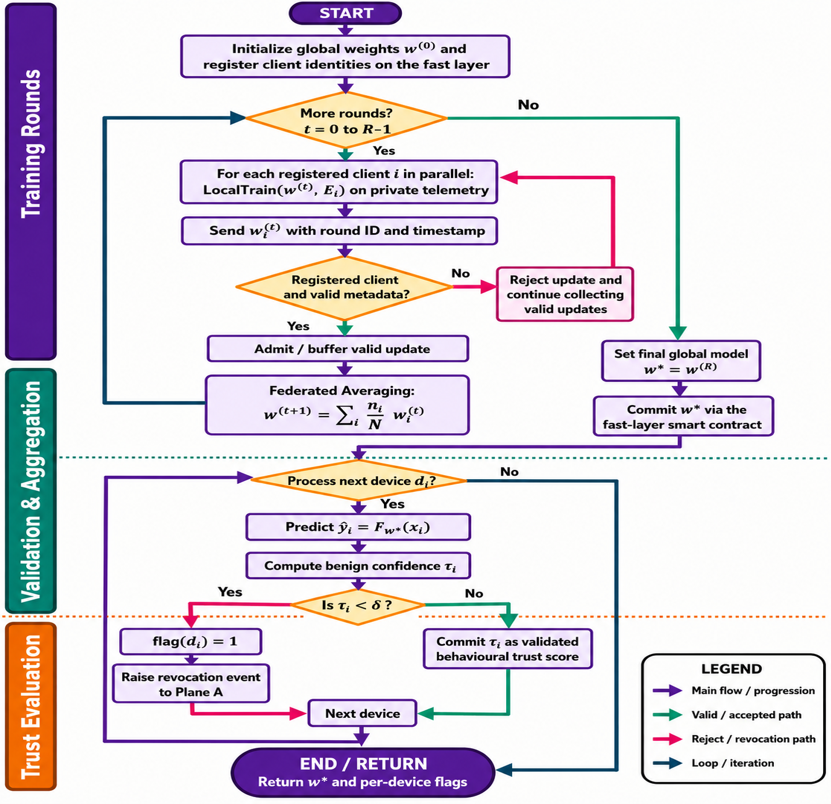
\includegraphics[width=\textwidth]{figures/Picture14.PNG}
  \caption{Operational flow of the federated trust-model training and behavioural commitment procedure.} 
  \label{fig:strata-train-flow}
\end{figure}

The trained engine is deliberately small, which is what allows continuous scoring within an edge budget. Its parameter count, layer configuration, and training settings are summarised in Table~\ref{tab:strata-hyper}, together with the trust threshold $\delta$ that fixes the flag rule of Equation~\eqref{eq:strata-flag}.

\begin{table}[t]
  \centering
  \footnotesize
  \setlength{\tabcolsep}{6pt}
  \renewcommand{\arraystretch}{1.25}
  \caption{Configuration of the trimmed CNN--LSTM trust engine and its trust-scoring rule. Model and training values are reused from the lightweight federated design; the final row states the trust-scoring output and flag threshold specific to this stratum.}
  \label{tab:strata-hyper}
  \begin{tabular}{@{}ll@{}}
    \toprule
    \textbf{Configuration item} & \textbf{Value} \\
    \midrule
    Model type              & 1-D CNN--LSTM \\
    Convolutional layers    & 16, 32 filters (kernel size 3) \\
    LSTM units              & 32 \\
    Dense layer             & 64 neurons + softmax output \\
    Activation              & ReLU (conv), softmax (output) \\
    Optimiser               & Adam \\
    Learning rate           & $1\times10^{-3}$ \\
    Batch size              & 64 \\
    Local epochs per round  & 5 \\
    Loss                    & categorical cross-entropy \\
    Dropout                 & 0.2 after the LSTM layer \\
    Trainable parameters    & 41{,}762 \\
    \addlinespace
    Trust score $q_i$    & benign-class confidence, $q_i\in[0,1]$ \\
    Flag rule               & $\text{flag}(d_i)=\mathbf{1}[q_i<\delta]$, threshold $\delta$ \\
    \bottomrule
  \end{tabular}
\end{table}
Kept to this size, the engine sustains continuous behavioural scoring on constrained hardware while producing a decision at the rate the fast layer requires. The verdict it commits is accurate but, once written, no longer alterable at the device, which is the property the next two strata build upon: Section~\ref{sec:strata-anchor} finalises and anchors these commitments, and Section~\ref{sec:strata-identity} converts a raised flag into an accountable revocation.


\section{The Consensus and Public-Anchoring Strata}
\label{sec:strata-anchor}

A behavioural verdict acquires no authority at the moment it is computed. Until it has been ordered against every other verdict in the network, accepted by a quorum that no single participant controls, and placed on a substrate that the accused device and its operator cannot rewrite, it remains a local opinion held by the gateway that produced it. The two upper strata of STRATA supply exactly those properties, and they supply them in sequence. The consensus and coordination stratum finalises the verdict inside the permissioned domain at a latency compatible with industrial control loops, and the public anchoring stratum carries a compact proof of that finalised record across the trust boundary onto a substrate whose write history lies beyond the reach of the consortium itself.

The division of labour is what keeps the arrangement affordable. Finalisation is frequent and cheap; anchoring is infrequent and expensive; assigning each class of event to the layer whose economics match its frequency is the operational content of trust-partitioning. Table~\ref{tab:strata-upper} sets the two strata against the properties each is required to deliver, and makes plain why neither could absorb the responsibilities of the other.

\begin{table}[t]
  \centering
  \footnotesize
  \setlength{\tabcolsep}{5pt}
  \renewcommand{\arraystretch}{1.3}
  \caption{Operational characteristics assigned to the consensus and public-anchoring strata, and the reason each property is unattainable on the other layer.}
  \label{tab:strata-upper}
  \begin{tabularx}{\textwidth}{@{}
      >{\raggedright\arraybackslash}p{2.9cm}
      >{\raggedright\arraybackslash}p{3.2cm}
      >{\raggedright\arraybackslash}p{3.2cm}
      >{\raggedright\arraybackslash}X@{}}
    \toprule
    \textbf{Property} & \textbf{Stratum~2 (consensus)} & \textbf{Stratum~3 (anchoring)} & \textbf{Reason for the split} \\
    \midrule
    Event frequency
      & Every behavioural verdict
      & One commitment per epoch
      & Per-event public writes are unaffordable at industrial verdict rates \\
    Settlement
      & Deterministic, final on commit
      & Probabilistic, subject to confirmation depth
      & Control actions cannot wait out a confirmation window \\
    Write authority
      & Consortium validators
      & Outside consortium administration
      & An operator-controlled ledger cannot attest to operator conduct \\
    Content exposed
      & Records and evidence bundles
      & Digests and hashed identifiers only
      & Payload disclosure would create a surface the deployment does not have today \\
    Cost driver
      & Signature verification per block
      & Transaction fee per commitment
      & Compute is elastic inside the plant; public fees are not \\
    \bottomrule
  \end{tabularx}
\end{table}

Figure~\ref{fig:strata-ecosystem} shows the five components that realise both strata and the paths along which records travel between them. Records enter at NSL-L2, where the behavioural stratum executes and where verdict digests are assembled. Ordering and acceptance occur at NSL-L1 under the PoA$^2$ acceptance rule, with SAM+ regulating the rate at which blocks are produced so that the permissioned chain neither starves under light industrial load nor saturates during an alarm storm. Only after a block is final does any material leave the permissioned domain, and what leaves is a digest, never a payload, which is the concrete enforcement of Theorem~\ref{thm:verifiability}.

\begin{figure}[t]
  \centering
  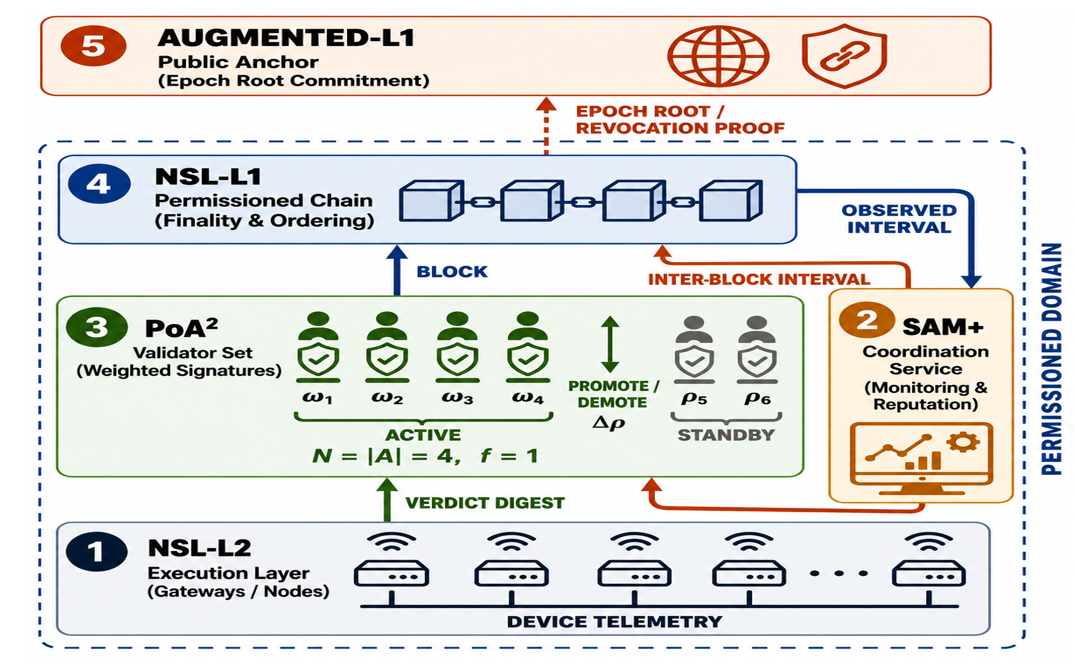
\includegraphics[width=\textwidth]{figures/Picture17.png}
  \caption{Component ecosystem realising the consensus and public-anchoring strata, comprising the SAM+ coordination service, the PoA$^2$ validator set, the NSL-L2 execution layer, the NSL-L1 permissioned chain, and the Augmented-L1 public anchor. Adapted from the published lightweight federated design~\cite{amadi2026lightweight}.}
  \label{fig:strata-ecosystem}
\end{figure}

\subsection{Consensus and Coordination}
\label{sec:strata-consensus}
Acceptance at the permissioned layer is decided by weighted authority rather than by expended work. Each validator $i$ in the active set $\mathcal{A}$ carries an authority weight $\omega_i$ that encodes both its institutional standing in the consortium and its observed operational reliability. A candidate block $B$ is committed when the weighted signatures it carries clear a fixed acceptance threshold:
\begin{equation}
\label{eq:poa2-accept}
\sum_{i \in \mathcal{A}} \omega_i \, \mathrm{sig}_i(B) \;\geq\; \theta ,
\end{equation}
where $\mathrm{sig}_i(B) \in \{0,1\}$ indicates whether validator $i$ signed $B$, $\omega_i \in [0,1]$ is the normalised authority weight of validator $i$, and $\theta$ is the acceptance threshold, set so that commitment requires a supermajority of weighted authority rather than a simple majority of nodes.

The reliability component of $\omega_i$ is not a static grant. It is tracked as an exponentially weighted moving average over the recent signing history of each validator, so that a node which is nominally authorised but persistently absent loses influence without requiring an administrative intervention:
\begin{equation}
\label{eq:poa2-reliability}
\rho_i(t) \;=\; \frac{\sum_{k=1}^{K} \gamma^{\,K-k} \, \mathrm{sig}_i(k)}{\sum_{k=1}^{K} \gamma^{\,K-k}} ,
\end{equation}
where $\rho_i(t) \in [0,1]$ is the reliability of validator $i$ at time $t$, $\mathrm{sig}_i(k)$ indicates whether validator $i$ signed block $k$, $K$ is the length of the observation window, and $\gamma \in (0,1)$ is the decay factor that weights recent participation above historical participation.

Reliability governs membership as well as influence. Validators whose reliability falls are demoted to the standby set $\mathcal{S}$, and standby nodes with sustained availability are promoted in their place. The exchange is triggered by a gap condition that prevents the active set from drifting into a state where a standby node is measurably more dependable than a serving one:
\begin{equation}
\label{eq:poa2-gap}
\max_{j \in \mathcal{S}} \rho_j(t) \;-\; \min_{i \in \mathcal{A}} \rho_i(t) \;<\; \Delta_\rho ,
\end{equation}
where $\mathcal{S}$ is the standby set, $\mathcal{A}$ is the active set, and $\Delta_\rho$ is the admissible reliability gap. When the condition is violated, the least reliable active validator is replaced by the most reliable standby validator, which gives the validator set a self-healing property without opening membership to unvetted participants.

Because authority is assigned rather than mined, agreement is deterministic and a committed block is final on commitment. There is no probabilistic settlement period during which a competing fork might displace an accepted verdict, and consequently no confirmation depth that industrial applications must wait out before acting on a revocation. The safety margin of the arrangement follows from the Byzantine bound applied to the active set:
\begin{equation}
\label{eq:poa2-fault}
f \;=\; \left\lfloor \frac{N-1}{2} \right\rfloor , \qquad N \;\geq\; 2f + 1 ,
\end{equation}
where $N = |\mathcal{A}|$ is the number of active validators and $f$ is the maximum number of simultaneously faulty or unavailable validators the layer tolerates while still admitting blocks. The bound is weaker than the $N \geq 3f+1$ requirement of open Byzantine agreement, and deliberately so. Validator identity is known and misbehaviour is attributable, which converts an anonymous adversary problem into an accountable one and permits the smaller quorum that constrained deployments can realistically staff.

Block production is regulated by the SAM+ coordination service, which adjusts the effort required to produce a block in response to observed network conditions rather than holding it at a fixed value. Industrial traffic is bursty by nature, and a fixed interval either wastes capacity during quiet periods or accumulates a backlog when an incident causes many gateways to report at once. The regulation objective is a bounded inter-block interval across both regimes:
\begin{equation}
\label{eq:sam-band}
T_{\min} \;\leq\; \bar{T}_{w} \;\leq\; T_{\max} ,
\end{equation}
where $\bar{T}_{w}$ is the mean inter-block interval observed over a sliding window $w$, and $T_{\min}$ and $T_{\max}$ bound the admissible interval. Holding the observed mean inside the band is what allows the behavioural stratum to treat finalisation latency as a bounded quantity when scheduling its own commitment step, and it is the property against which the layer is later measured. Table~\ref{tab:consensus-params} collects the parameters that govern the stratum, the constraint each one expresses, and the effect of moving it.

\begin{table}[t]
  \centering
  \footnotesize
  \setlength{\tabcolsep}{5pt}
  \renewcommand{\arraystretch}{1.3}
  \caption{Parameters governing the consensus and coordination stratum, with the constraint each expresses and the consequence of altering it.}
  \label{tab:consensus-params}
  \begin{tabularx}{\textwidth}{@{}
      >{\raggedright\arraybackslash}p{1.6cm}
      >{\raggedright\arraybackslash}p{4.0cm}
      >{\raggedright\arraybackslash}p{2.6cm}
      >{\raggedright\arraybackslash}X@{}}
    \toprule
    \textbf{Symbol} & \textbf{Quantity} & \textbf{Governs} & \textbf{Effect of increase} \\
    \midrule
    $\theta$
      & Weighted acceptance threshold
      & Block acceptance
      & Stronger safety, reduced liveness under validator absence \\
    $\gamma$
      & Reliability decay factor
      & Reliability tracking
      & Longer memory of past participation, slower demotion \\
    $\Delta_\rho$
      & Admissible reliability gap
      & Set membership
      & Fewer set changes, greater tolerance of degraded validators \\
    $N$
      & Active validator count
      & Fault tolerance
      & Higher fault tolerance, higher signature-verification cost per block \\
    $T_{\max}$
      & Upper bound on inter-block interval
      & Block cadence
      & Lower block overhead, higher worst-case finalisation latency \\
    \bottomrule
  \end{tabularx}
\end{table}

\subsection{Public Anchoring}
\label{sec:strata-public}
Everything described so far is internal to a consortium that the plant operator controls, and that control is precisely the residual risk. A permissioned ledger operated by the party whose conduct is under audit offers no protection against a coordinated rewrite by that party. The public anchoring stratum removes the possibility by committing periodic digests of the permissioned history to a substrate outside consortium administration, so that any retrospective alteration inside the consortium becomes detectable by comparison against a record the consortium cannot edit.

The public layer exposes a narrow interface, and the narrowness is deliberate. Admission binds an identifier to a credential commitment without disclosing the credential:
\begin{equation}
\label{eq:register}
\mathrm{Register}(\mathrm{id}) \;\longmapsto\; \big\langle \, H(\mathrm{id}), \; H(\mathrm{pk}), \; \mathrm{dom}, \; t_e \, \big\rangle ,
\end{equation}
where $H(\mathrm{id})$ is the digest of the device identifier, $H(\mathrm{pk})$ is the digest of the public credential issued at enrolment, $\mathrm{dom}$ names the permissioned domain that vouches for the device, and $t_e$ is the enrolment timestamp. A relying party already in possession of an identifier and credential can confirm admission by recomputing both digests; a party in possession of neither learns only that some device was admitted, which is what prevents the public record from becoming an inventory of the plant.

Withdrawal is the mirror of admission, and it is the one class of event that is never deferred. When the behavioural stratum drives a device trust score below the revocation threshold $\tau$, the finding is not merely recorded, it is published, because its purpose is to inform parties outside the consortium that the credential is no longer honoured:
\begin{equation}
\label{eq:revoke}
\mathrm{Revoke}(\mathrm{id}) \;\Longrightarrow\; \big\langle \, H(\mathrm{id}), \; H(\pi), \; t_r \, \big\rangle ,
\end{equation}
where $H(\pi)$ is the digest of the evidence bundle supporting the revocation and $t_r$ is the revocation timestamp. The evidence bundle itself remains inside the permissioned domain and is disclosed only to parties with cause. What becomes public is the fact of revocation together with a commitment binding it to evidence that cannot subsequently be substituted, so a later dispute cannot be settled by producing a more convenient bundle. Publication succeeds only for a revocation block that has already cleared the weighted acceptance threshold, which is the point at which the two strata meet:
\begin{equation}
\label{eq:publish-revocation}
\mathrm{publishRevocation}\big(H(\mathrm{id}), H(\pi)\big) \;=\;
\begin{cases}
\text{committed}, & \text{if } \displaystyle\sum_{i \in \mathcal{A}} \omega_i \, \mathrm{sig}_i(B_r) \geq \theta, \\[6pt]
\text{rejected}, & \text{otherwise},
\end{cases}
\end{equation}
where $B_r$ is the revocation block carrying the withdrawal tuple. No single gateway, and no single validator, can withdraw a device unilaterally, and equally no operator can suppress a revocation that the validator set has already accepted.
Routine verdicts are handled differently, because publishing each one at the rate industrial monitoring produces them would exhaust any realistic transaction budget. They are aggregated by epoch, and the epoch is the unit that makes the arrangement viable.

\begin{definition}[Anchoring epoch]
\label{def:epoch}
An anchoring epoch $\mathcal{E}_k$ is the ordered set of finalised verdict digests $\{H_1, H_2, \ldots, H_E\}$ produced at the permissioned layer between two successive public commitments, where $E = |\mathcal{E}_k|$ is the epoch span.
\end{definition}

The digests in an epoch are combined into a single value by binary hashing, and that value alone crosses the boundary:
\begin{equation}
\label{eq:merkle-root}
R_k \;=\; \mathrm{MerkleRoot}\!\left(H_1, H_2, \ldots, H_E\right) ,
\end{equation}
where $R_k$ is the epoch root committed publicly and $H_j$ is the digest of the $j$-th finalised record in the epoch. Membership of any individual record in the anchored epoch is subsequently demonstrable by supplying $\lceil \log_2 E \rceil$ sibling hashes, so selective verification of one device history never requires disclosure of, or access to, the remaining records in the epoch. The public commitment records the root together with the minimal metadata needed to locate and interpret it:
\begin{equation}
\label{eq:anchor-tuple}
\mathcal{C}_k \;=\; \big\langle \, k, \; R_k, \; \mathrm{dom}, \; v, \; t_k \, \big\rangle ,
\end{equation}
where $k$ identifies the epoch, $R_k$ is the epoch root, $\mathrm{dom}$ names the permissioned domain of origin, $v$ is the schema version under which the records were serialised, and $t_k$ is the commitment timestamp. No device identifier, no feature vector, and no trust score appears in the commitment, which is why anchoring adds no disclosure surface to a deployment.

Verification is a single comparison. An auditor holding a claimed record recomputes its digest, recomputes the root along the supplied Merkle path, and tests the result against the anchored value:
\begin{equation}
\label{eq:anchor-verify}
V \;=\; \mathbf{1}\!\left[\, \hat{R}_k \;=\; R_k^{\mathrm{chain}} \,\right] ,
\end{equation}
where $\hat{R}_k$ is the root recomputed from the record and its Merkle path, $R_k^{\mathrm{chain}}$ is the root read from the public commitment, and $V = 1$ certifies that the record is exactly the one the consortium finalised in epoch $k$. A single altered bit anywhere in the epoch produces $V = 0$, and the alteration is detectable by any party, including one with no standing inside the consortium.

Two parameters govern the cadence, and they pull against each other. The epoch closes on whichever of a count bound and a time bound is reached first:
\begin{equation}
\label{eq:epoch-close}
\Delta t_{\mathrm{anchor}} \;=\; \min\!\left( \frac{E}{\lambda}, \; T_{\mathrm{epoch}} \right) ,
\end{equation}
where $\lambda$ is the verdict arrival rate, $E$ is the epoch span, and $T_{\mathrm{epoch}}$ is the maximum tolerated interval of unanchored exposure. The time bound is what protects a quiet installation: without it, a plant producing few verdicts would leave its history unanchored for arbitrarily long simply because the count never filled. Figure~\ref{fig:strata-epoch} shows the resulting cadence, with routine verdicts accumulating toward an epoch boundary while a sub-threshold verdict leaves immediately by the revocation path. The economic argument for epoch-based anchoring is stated directly.
\begin{figure}[t]
  \centering
  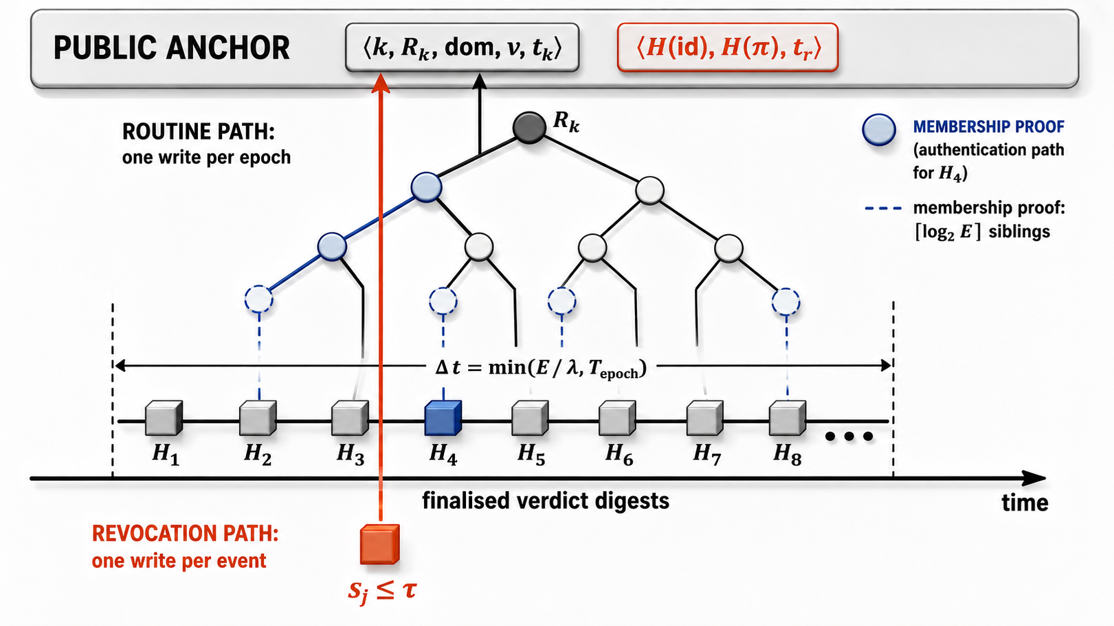
\includegraphics[width=\textwidth]{figures/Picture18.png}
  \caption{Anchoring cadence at the public stratum. Finalised verdict digests
accumulate across an epoch and are aggregated into a single root committed
once per epoch, while a verdict falling below the threshold $\tau$ is
published immediately by the revocation path and anchored in the epoch as
well.}
  \label{fig:strata-epoch}
\end{figure}



\begin{proposition}
\label{prop:anchor-rate}
For a verdict arrival rate $\lambda$ and an epoch span $E$, the public-layer write rate induced by routine anchoring is $\lambda / E$, and the evidence retained for any individual verdict is $\lceil \log_2 E \rceil$ hash values.
\end{proposition}

\begin{proof}
Each epoch consumes $E$ verdicts and produces exactly one commitment, so commitments are emitted at rate $\lambda / E$. Membership of a leaf in a balanced binary hash tree of $E$ leaves is witnessed by the sibling hash at each level, of which there are $\lceil \log_2 E \rceil$. Neither quantity depends on the size of the underlying record.
\end{proof}

The consequence is that public-layer cost is decoupled from behavioural event volume. Raising the epoch span reduces anchoring cost linearly while increasing proof size only logarithmically, and the operator tunes the span against the maximum acceptable interval of unanchored exposure rather than against a fixed transaction budget. Revocations are excluded from the aggregation and therefore from the reduction, which is the correct trade: the events that justify a per-event public write are exactly the events a relying party must learn about without waiting.
Table~\ref{tab:device-lifecycle} sets out the states a device occupies between admission and revocation, together with the transition that moves it and the stratum at which the transition is observed.

\begin{table}[t]
  \centering
  \footnotesize
  \setlength{\tabcolsep}{5pt}
  \renewcommand{\arraystretch}{1.3}
  \caption{Device lifecycle states, transition conditions, and the stratum at which each transition is observed.}
  \label{tab:device-lifecycle}
  \begin{tabularx}{\textwidth}{@{}
      >{\raggedright\arraybackslash}p{2.3cm}
      >{\raggedright\arraybackslash}X
      >{\raggedright\arraybackslash}p{3.6cm}
      >{\raggedright\arraybackslash}p{2.2cm}@{}}
    \toprule
    \textbf{State} & \textbf{Condition} & \textbf{Transition trigger} & \textbf{Observed at} \\
    \midrule
    Unregistered
      & No credential bound to the identifier
      & Enrolment and credential issue
      & Plane~A \\
    Active
      & Trust score above the operating band
      & Score falls into the monitored band
      & Stratum~1 \\
    Monitored
      & Score degraded but above $\tau$
      & Sustained degradation or a detection event
      & Stratum~1 \\
    Flagged
      & Score at or below $\tau$, pending finalisation
      & Revocation block reaches the acceptance threshold
      & Stratum~2 \\
    Revoked
      & Credential withdrawn and published
      & Terminal; re-entry requires re-enrolment
      & Stratum~3 \\
    \bottomrule
  \end{tabularx}
\end{table}

The lifecycle is monotone in one direction only. A device may recover from Monitored to Active while its score remains above $\tau$, but no transition returns a device from Revoked to Active, because the credential itself has been withdrawn and its replacement is a fresh enrolment producing a fresh identifier. The asymmetry is what makes a published revocation meaningful: a relying party observing the record on the public substrate does not have to establish whether the finding was later quietly reversed inside the consortium. Figure~\ref{fig:strata-crosschain} shows the crossing itself, from permissioned finalisation on one substrate to the commitment recorded on the other.

\begin{figure}[t]
  \centering
  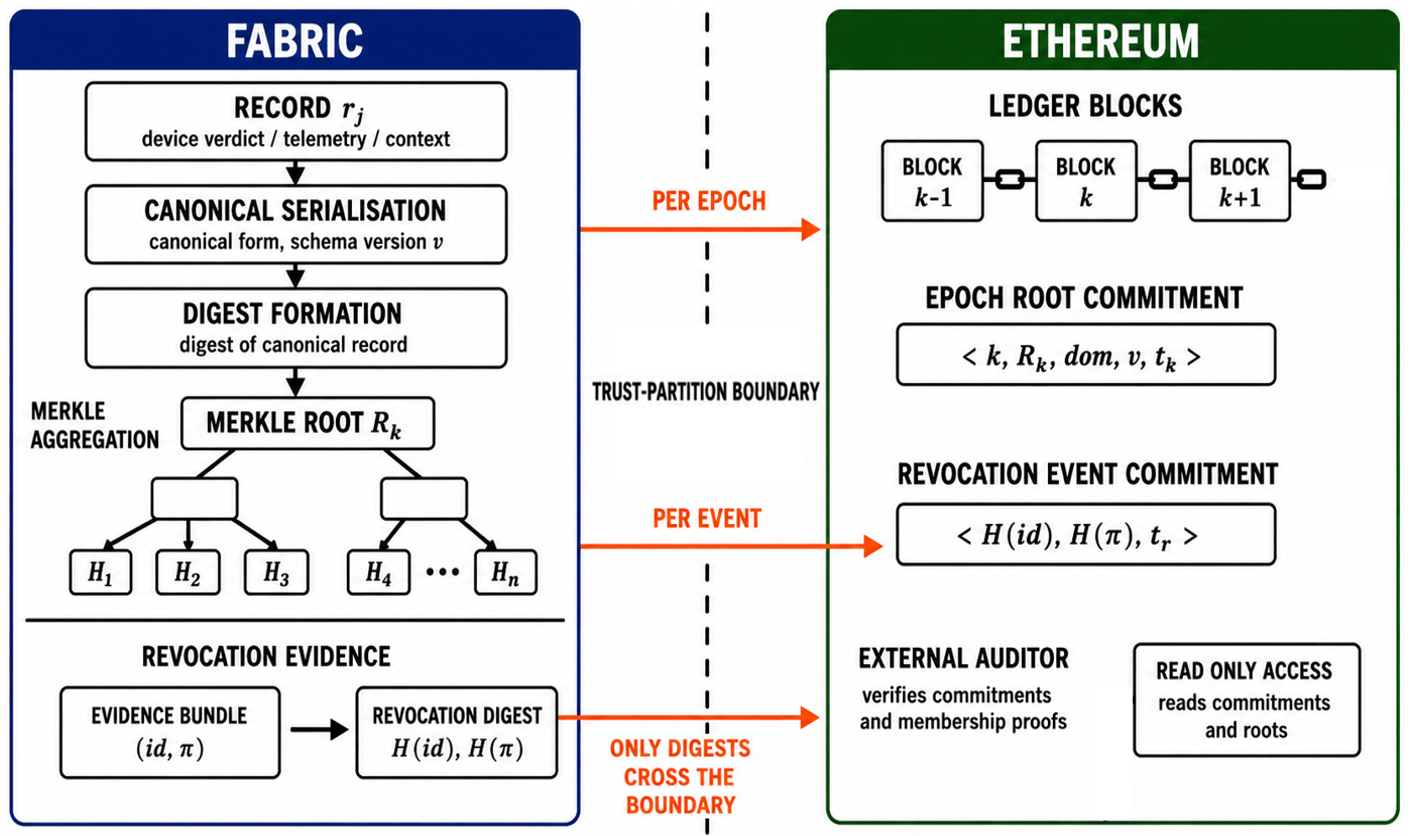
\includegraphics[width=0.92\textwidth]{figures/Picture19.PNG}
  \caption{Cross-boundary commitment path from the permissioned execution and consensus layers to the public anchor, showing digest formation, epoch aggregation, and the revocation channel. Adapted from the published hybrid-ledger cross-chain design~\cite{amadi2026symmetric}.}
  \label{fig:strata-crosschain}
\end{figure}

Algorithm~\ref{alg:strata-anchor} states the production procedure. It accepts the finalised verdict digests that the behavioural stratum produces, aggregates them by epoch, and diverts any record carrying a sub-threshold trust score into the revocation channel rather than the aggregation channel.

\begin{algorithm}[t]
\caption{Epoch anchoring and revocation-proof commitment}
\label{alg:strata-anchor}
\begin{algorithmic}[1]
\Require Stream of finalised records $\{r_j\}$ with trust scores $s_j$; epoch span $E$; epoch timeout $T_{\mathrm{epoch}}$; revocation threshold $\tau$; acceptance threshold $\theta$
\Ensure Public commitments $\{\mathcal{C}_k\}$ and published revocation records
\State $\mathcal{E} \gets \emptyset$; \; $k \gets 0$; \; start epoch timer
\For{each finalised record $r_j$ arriving from Stratum~2}
  \State $H_j \gets H(\mathrm{canonical}(r_j))$
  \If{$s_j \leq \tau$}
    \State $\pi_j \gets$ evidence bundle for $r_j$, retained in the permissioned domain
    \State assemble revocation block $B_r$ carrying $\langle H(\mathrm{id}_j), H(\pi_j), t_r \rangle$
    \If{$\sum_{i \in \mathcal{A}} \omega_i \, \mathrm{sig}_i(B_r) \geq \theta$}
      \State publish the tuple to the public anchor
      \State set lifecycle state of $\mathrm{id}_j$ to Revoked
    \EndIf
  \EndIf
  \State $\mathcal{E} \gets \mathcal{E} \cup \{H_j\}$
  \If{$|\mathcal{E}| = E$ \textbf{or} epoch timer $\geq T_{\mathrm{epoch}}$}
    \State $R_k \gets \mathrm{MerkleRoot}(\mathcal{E})$
    \State commit $\mathcal{C}_k \gets \langle k, R_k, \mathrm{dom}, v, t_k \rangle$ to the public anchor
    \State retain Merkle paths for the members of $\mathcal{E}$ in the permissioned domain
    \State $\mathcal{E} \gets \emptyset$; \; $k \gets k+1$; \; reset epoch timer
  \EndIf
\EndFor
\State \Return $\{\mathcal{C}_k\}$ and the published revocation records
\end{algorithmic}
\end{algorithm}

The audit procedure that consumes those commitments is stated separately in Algorithm~\ref{alg:strata-verify}, because the party that runs it is not the party that produced the record. An auditor requires the record under examination, the Merkle path retained beside it, and read access to the public substrate. No credential, no consortium membership, and no cooperation from the operator beyond release of the record is needed, which is the property that distinguishes anchoring from internal logging.

\begin{algorithm}[t]
\caption{Independent verification of an anchored record}
\label{alg:strata-verify}
\begin{algorithmic}[1]
\Require Claimed record $r$; Merkle path $\Pi$; epoch index $k$; read access to the public anchor
\Ensure Verdict $V \in \{0,1\}$ on the integrity of $r$
\State $\hat{H} \gets H(\mathrm{canonical}(r))$ \Comment{same serialisation rules and schema version $v$}
\State $\hat{R}_k \gets \hat{H}$
\For{each sibling $h \in \Pi$, from leaf to root}
  \State $\hat{R}_k \gets H(\hat{R}_k \,\|\, h)$ in the order recorded by the path
\EndFor
\State read $\mathcal{C}_k = \langle k, R_k^{\mathrm{chain}}, \mathrm{dom}, v, t_k \rangle$ from the public anchor
\If{schema version of $r$ $\neq v$}
  \State \Return $V \gets 0$ \Comment{serialisation mismatch invalidates the comparison}
\EndIf
\State $V \gets \mathbf{1}[\hat{R}_k = R_k^{\mathrm{chain}}]$
\State \Return $V$
\end{algorithmic}
\end{algorithm}

Two properties of the pair deserve emphasis, because they are the properties an evaluator will test. First, the public substrate receives no data whose disclosure could harm the operator: the aggregation channel emits roots, and the revocation channel emits hashed identifiers and evidence commitments, so the anchoring stratum adds durability without adding exposure. Second, the cost the operator pays for that durability is bounded and tunable by a single parameter, the routine public write rate holding at $\lambda/E$ independent of how much behavioural traffic the lower strata process. The measured expression of both properties, in anchoring latency and in per-device overhead on constrained hardware, is reported in Chapter~\ref{Chapter_5}.

What remains unspecified is the credential that binds a device to the identifier carried in the registration and withdrawal records, the law by which a trust score decays toward the threshold that triggers withdrawal, and the cryptographic substrate that must keep credential and anchored commitment meaningful once classical hardness assumptions no longer hold. Those are the concerns of the two cross-cutting planes, treated in Section~\ref{sec:strata-identity}.


\section{Quantum-Resilient Identity and Revocation}
\label{sec:strata-identity}

The three strata described so far assume two things they do not themselves provide. Every record carries a device identifier, and the whole apparatus of behavioural scoring, finalisation and anchoring is worthless if that identifier can be forged, cloned across devices, or reused after withdrawal. Every digest, signature and key exchange rests on a hardness assumption, and a deployment expected to remain in service for fifteen years cannot assume that the assumption holding today still holds at decommissioning. Neither concern belongs to a single stratum. Identity is asserted at the edge, evaluated at the behavioural layer, finalised at the consensus layer and published at the anchor; cryptographic strength is required at each of those points and at the boundaries between them. Both are therefore carried as planes cutting vertically through the stack rather than as layers stacked upon it.

Plane~A binds a physical device to an identifier and governs the withdrawal of that binding. Plane~B supplies the cryptographic substrate on which the binding, and every commitment derived from it, is expressed. Table~\ref{tab:planes-matrix} states what each plane contributes at each stratum, and the pattern in the table is the justification for treating them as planes: no row is empty, and no stratum could supply for itself what the planes supply.

\begin{table}[t]
  \centering
  \footnotesize
  \setlength{\tabcolsep}{5pt}
  \renewcommand{\arraystretch}{1.3}
  \caption{Contribution of the two cross-cutting planes at each stratum of the architecture.}
  \label{tab:planes-matrix}
  \begin{tabularx}{\textwidth}{@{}
      >{\raggedright\arraybackslash}p{3.0cm}
      >{\raggedright\arraybackslash}X
      >{\raggedright\arraybackslash}X@{}}
    \toprule
    \textbf{Stratum} & \textbf{Plane~A: identity and revocation} & \textbf{Plane~B: post-quantum substrate} \\
    \midrule
    Behavioural trust
      & Supplies the identifier under which observations are attributed and scores accumulated
      & Protects model updates in transit between gateway and aggregator \\
    Consensus and coordination
      & Supplies the credential a validator checks before admitting a record for ordering
      & Protects the session keys under which validators exchange candidate blocks \\
    Public anchoring
      & Supplies the hashed identifier published on withdrawal, and the evidence commitment bound to it
      & Determines how long an anchored commitment remains meaningful against a future adversary \\
    \bottomrule
  \end{tabularx}
\end{table}

\subsection{Plane A: Identity Derivation and Trust Decay}
\label{sec:plane-a}

An identifier that is assigned administratively can be reassigned administratively, which places the operator inside the trust boundary of every claim made about a device. Deriving the identifier from physical entropy captured at the device removes that discretion. The identifier is fixed at enrolment as the digest of three concatenated components:
\begin{equation}
\label{eq:identity-derive}
\mathrm{id}_i \;=\; H\big( e_i \,\|\, t_i \,\|\, d_i \big) ,
\end{equation}
where $e_i$ is a sample drawn from the device entropy source, $t_i$ is the enrolment timestamp, and $d_i$ is a device-specific token held in the secure element. The entropy sample makes the identifier unpredictable to an adversary who knows the device model and enrolment time; the timestamp makes a replayed enrolment produce a distinct identifier; and the device token binds the result to hardware that cannot be relocated without physical access. None of the three is sufficient alone, and the digest is one-way, so publishing the identifier discloses nothing about the entropy sample that produced it.

\begin{definition}[Device credential]
\label{def:credential}
A device credential is the pair $\langle \mathrm{id}_i, \mathrm{pk}_i \rangle$ formed at enrolment, where $\mathrm{id}_i$ is derived from device entropy and $\mathrm{pk}_i$ is the public key of the keypair generated in the secure element. The credential is valid while the trust score of the device remains above the revocation threshold, and terminally invalid thereafter.
\end{definition}

Table~\ref{tab:entropy-sources} lists the sources available on constrained industrial hardware, distinguishing what a given class of device can actually offer from what the derivation requires of it.

\begin{table}[t]
  \centering
  \footnotesize
  \setlength{\tabcolsep}{5pt}
  \renewcommand{\arraystretch}{1.3}
  \caption{Entropy sources available for identifier derivation on constrained industrial hardware.}
  \label{tab:entropy-sources}
  \begin{tabularx}{\textwidth}{@{}
      >{\raggedright\arraybackslash}p{2.8cm}
      >{\raggedright\arraybackslash}p{2.2cm}
      >{\raggedright\arraybackslash}p{3.4cm}
      >{\raggedright\arraybackslash}X@{}}
    \toprule
    \textbf{Source} & \textbf{Class} & \textbf{Availability} & \textbf{Suitability for one-time derivation} \\
    \midrule
    Hardware TRNG in secure element
      & Physical
      & Security-class microcontrollers; absent from legacy field devices
      & Preferred wherever present; no debiasing or conditioning required \\
    Ring-oscillator jitter
      & Physical
      & FPGA and selected microcontroller families
      & Throughput well above what a single enrolment consumes \\
    SRAM power-up state
      & Physical
      & Any device exposing uninitialised SRAM
      & One sample per power cycle; device-unique but requires debiasing \\
    Sensor noise floor
      & Environmental
      & Universal on instrumented devices
      & Serviceable fallback; entropy rate varies with process conditions \\
    Seeded software generator
      & Simulated
      & Any platform
      & Architectural validation only; unsuitable for a fielded credential \\
    \bottomrule
  \end{tabularx}
  \vspace{2pt}
  \footnotesize\raggedright
  Identifier derivation in the present realisation is seeded from the software source in the final row. The four physical and environmental sources are specified as deployment options and are not exercised here.
\end{table}

The construction consumes the entropy sample as an opaque bit string, so substituting a hardware source at deployment changes the quality of that sample and nothing else: the derivation, the storage cost of the resulting identifier, and every subsequent lifecycle operation are unaffected. What the present realisation establishes is that those operations behave as specified end to end; what it leaves to a fielded deployment is the entropy quality the chosen source actually delivers.

Withdrawal is driven by accumulated behavioural evidence rather than by a single detection. The trust score of a device is updated once per observation window by blending its previous value with the evidence from the current window:
\begin{equation}
\label{eq:trust-decay}
s_i(t+1) \;=\; \beta \, s_i(t) \;+\; (1-\beta) \, q_i(t) ,
\end{equation}
where $s_i(t) \in [0,1]$ is the trust score of device $i$ at window $t$, $q_i(t) \in [0,1]$ is the behavioural evidence produced for that window by the trust-scoring stratum, and $\beta \in (0,1)$ is the retention factor governing how strongly past behaviour resists present evidence. A high retention factor makes the score slow to fall, which suppresses reaction to transient noise at the cost of delaying response to a genuine compromise; a low factor inverts both properties. Withdrawal follows once the score falls to or below the revocation threshold $\tau$, at which point the credential is terminally invalid. Because the update is a convex combination, the score cannot leave the unit interval, and a device supplying uniformly clean evidence converges upward toward unity rather than accumulating unbounded credit for good behaviour.

A second, independent trigger bounds the response to abrupt compromise. A streak counter $S_i(t)$ records the number of consecutive windows in which the behavioural score $q_i(t)$ has fallen below the flag threshold $\delta$, and is reset by any window of normal behaviour. Withdrawal therefore follows when either condition is met,
\begin{equation}
\label{eq:revoke-condition}
\mathrm{Revoke}(\mathrm{id}_i) \iff s_i(t) \leq \tau \;\; \text{or} \;\; S_i(t) > \mu_S ,
\end{equation}
where $\mu_S$ is the streak limit. The threshold condition catches gradual degradation accumulated over many windows, while the streak condition catches a device that fails every window in succession before its score has had time to fall. The trust law may equally be realised in an additive form, in which each window credits or penalises the score by a fixed amount; that form shares the threshold semantics and the terminal withdrawal of Equation~\eqref{eq:trust-decay} but declines linearly rather than geometrically, and it is the form exercised in the isolation experiments of Chapter~\ref{Chapter_5}.

The delay this introduces between compromise and withdrawal is bounded, and the bound is what an operator needs in order to choose the retention factor.

\begin{proposition}
\label{prop:revocation-delay}
Let a device hold score $s_i(0) > \tau$ and thereafter supply evidence at a constant level $q < \tau$. The number of observation windows before withdrawal is
\[
k \;=\; \left\lceil \frac{\ln\!\big( (\tau - q) / (s_i(0) - q) \big)}{\ln \beta} \right\rceil .
\]
\end{proposition}

\begin{proof}
Writing the update as a deviation from the evidence level, $s_i(t+1) - q = \beta\,(s_i(t) - q)$, so $s_i(k) - q = \beta^{k}\,(s_i(0) - q)$. Withdrawal occurs at the least $k$ satisfying $s_i(k) \leq \tau$, that is $\beta^{k}(s_i(0) - q) \leq \tau - q$. Both sides are positive because $q < \tau < s_i(0)$, and $\ln \beta < 0$, so taking logarithms and dividing reverses the inequality and yields the stated expression on rounding up to a whole window.
\end{proof}

Two consequences follow. The first is a design guide: an operator who fixes an acceptable response time can solve the expression for the retention factor rather than tuning it by trial. The second is a limitation. Time to withdrawal grows without bound as the evidence level approaches the threshold from below, so an adversary degrading behaviour just far enough to sit marginally beneath it is withdrawn slowly. That strategy is defeated by detecting the degradation, not by accelerating the decay, since a decay steep enough to catch it would withdraw healthy devices on transient noise. The score is a filter over evidence rather than a detector in its own right, and responsibility for recognising the pattern sits with the behavioural stratum. Figure~\ref{fig:trust-decay} places the scoring loop in the wider credential lifecycle it governs.

\begin{figure}[t]
  \centering
  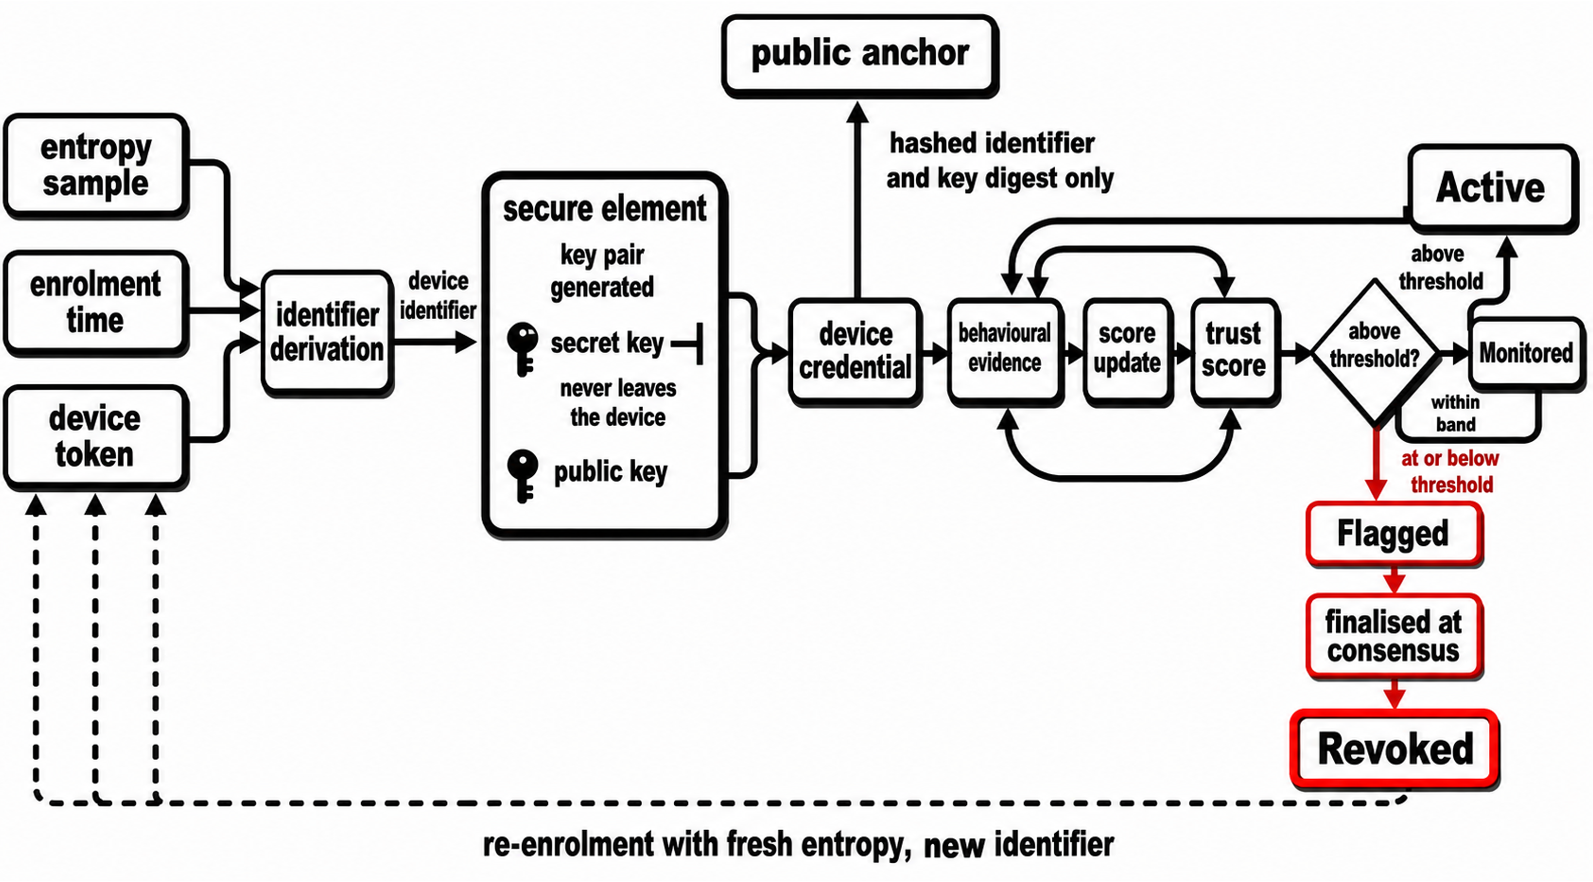
\includegraphics[width=\textwidth]{figures/Picture20.PNG}
  \caption{Credential mechanism of Plane~A, from entropy-seeded derivation and secure-element binding through the scoring loop to withdrawal. Withdrawal is terminal, and replacement requires re-enrolment under a fresh identifier.}
  \label{fig:trust-decay}
\end{figure}

Algorithm~\ref{alg:identity-lifecycle} sets out the full credential lifecycle, from enrolment through scoring to withdrawal and the handling of a replacement device.

\begin{algorithm}[t]
\caption{Credential issuance, decay and withdrawal}
\label{alg:identity-lifecycle}
\begin{algorithmic}[1]
\Require Device $i$ presenting entropy sample $e_i$ and device token $d_i$; retention factor $\beta$; revocation threshold $\tau$; initial score $s_0$
\Ensure Credential $\langle \mathrm{id}_i, \mathrm{pk}_i \rangle$ and its lifecycle state
\State $\mathrm{id}_i \gets H(e_i \,\|\, t_i \,\|\, d_i)$
\State generate keypair $(\mathrm{sk}_i, \mathrm{pk}_i)$ inside the secure element; $\mathrm{sk}_i$ never leaves it
\State register $\langle H(\mathrm{id}_i), H(\mathrm{pk}_i), \mathrm{dom}, t_i \rangle$ at the public anchor
\State $s_i \gets s_0$; \; state $\gets$ Active
\For{each observation window $t$}
  \State $q_i(t) \gets$ behavioural evidence from the trust-scoring stratum
  \State $s_i \gets \beta \, s_i + (1-\beta)\, q_i(t)$
  \State update streak counter $S_i$ \Comment{reset on a normal window}
  \If{$s_i \leq \tau$ \textbf{or} $S_i > \mu_S$}
    \State state $\gets$ Flagged; assemble evidence bundle $\pi_i$
    \State submit revocation for finalisation at the consensus stratum
    \If{revocation is committed}
      \State publish $\langle H(\mathrm{id}_i), H(\pi_i), t_r \rangle$; \; state $\gets$ Revoked
      \State \textbf{break} \Comment{terminal; the credential is not reinstated}
    \EndIf
  \ElsIf{$s_i$ below the operating band}
    \State state $\gets$ Monitored
  \Else
    \State state $\gets$ Active
  \EndIf
\EndFor
\State \Return $\langle \mathrm{id}_i, \mathrm{pk}_i \rangle$, state
\end{algorithmic}
\end{algorithm}

Replacement of a withdrawn device re-enters the procedure at the first line with a fresh entropy sample, producing an identifier unrelated to the withdrawn one. There is no reinstatement path, and there is no derivation linking the replacement to its predecessor, so an adversary observing the public record cannot establish that a newly admitted device occupies the position of a recently withdrawn one.

\subsection{Plane B: Post-Quantum Substrate}
\label{sec:plane-b}
A commitment anchored today is intended to remain checkable for the service life of the installation, and an industrial asset outlives several cryptographic generations. Two distinct exposures follow, and they have different urgencies. Confidentiality is exposed retroactively, because traffic captured now can be stored and decrypted once a capable adversary exists, so key establishment must be migrated before such an adversary appears rather than after. Integrity is exposed prospectively: a digest cannot be retrospectively forged into a commitment already published, so anchored records are threatened only from the point at which forgery becomes feasible.

Key establishment therefore adopts a lattice-based encapsulation mechanism in place of classical key agreement. The sender encapsulates against the recipient public key, obtaining a ciphertext to transmit and a shared secret to retain; the recipient recovers the same secret by decapsulating that ciphertext with the secret key held in its secure element. The shared secret never traverses the network in any form, and the ciphertext discloses nothing about it to an observer lacking the secret key.

The obstacle to deploying this on constrained hardware is size rather than speed. Lattice ciphertexts and public keys are substantially larger than their elliptic-curve counterparts, and on low-rate industrial radio links the transmission cost of that expansion dominates the computational cost of the primitive itself. A reversible compression is therefore applied to the ciphertext before transmission and inverted on receipt. The map is lossless with respect to the decapsulation input, so the shared secret recovered after inversion is identical to the one that would have been recovered from the uncompressed ciphertext, and the security argument for the underlying mechanism is unaffected. The reduction achieved and its effect on end-to-end handshake latency on constrained hardware are reported in Chapter~\ref{Chapter_5}.

Table~\ref{tab:pq-placement} records where each primitive sits in the architecture and which exposure it answers, together with the migration status of each position.

\begin{table}[t]
  \centering
  \footnotesize
  \setlength{\tabcolsep}{5pt}
  \renewcommand{\arraystretch}{1.3}
  \caption{Placement of cryptographic primitives across the architecture, the exposure each position carries, and its migration status in the present design.}
  \label{tab:pq-placement}
  \begin{tabularx}{\textwidth}{@{}
      >{\raggedright\arraybackslash}p{3.4cm}
      >{\raggedright\arraybackslash}p{2.9cm}
      >{\raggedright\arraybackslash}X
      >{\raggedright\arraybackslash}p{2.3cm}@{}}
    \toprule
    \textbf{Position} & \textbf{Primitive class} & \textbf{Exposure} & \textbf{Status} \\
    \midrule
    Device-to-gateway session
      & Lattice encapsulation
      & Retroactive: captured traffic decrypted later
      & Migrated \\
    Gateway-to-aggregator update transfer
      & Lattice encapsulation
      & Retroactive: model updates disclose local behaviour
      & Migrated \\
    Identifier derivation
      & Hash
      & Preimage resistance degrades by a square-root factor only
      & Adequate \\
    Record and epoch digests
      & Hash
      & Collision resistance sets the forgery horizon for anchored records
      & Adequate \\
    Validator block signatures
      & Digital signature
      & Prospective: forgery feasible only once a capable adversary exists
      & Migration item \\
    Device credential signatures
      & Digital signature
      & Prospective: forged credentials admit unauthorised devices
      & Migration item \\
    \bottomrule
  \end{tabularx}
\end{table}

Two rows of that table are marked as outstanding, and the reason is worth stating rather than leaving to inference. Signature migration multiplies key and signature sizes at every point where a block is signed and every point where a credential is presented, and unlike the session case those artefacts are stored rather than transmitted once. Sizing that cost against the storage budget of a field gateway is an engineering exercise the present design has not completed, and the prospective nature of the exposure makes deferral defensible in a way that deferring key establishment would not be. The hash positions carry no migration item because the known quantum advantage against preimage resistance is quadratic rather than exponential, which is absorbed by the digest lengths already in use.

\section{Cross-Substrate Instantiation and Setup}
\label{sec:strata-substrates}

An architecture demonstrated on one ledger and nowhere else invites a reasonable objection: that what has been shown is a property of that ledger rather than of the design built upon it. The objection is not academic. Permissioned and public substrates differ in their execution model, their finality semantics, their transaction economics and their identity assumptions, and a partition that survives only under one particular combination of those properties is an implementation detail dressed as a principle. Establishing that trust-partitioning is a property of the design requires realising the same partition twice, on substrates chosen for their difference rather than their similarity, and showing that the roles assigned to each stratum are discharged in both.

Two instantiations are used. The first realises all three strata on a purpose-built lightweight ledger with a native two-layer execution model, an authority-weighted consensus and a public anchor of its own. The second realises the identical partition on an enterprise pairing in which a permissioned chain provides execution and finalisation and a general-purpose public chain provides anchoring. The substrates were not chosen for convenience: one is a research ledger designed for constrained devices, the other a production stack with an installed base in industrial consortia, and their consensus mechanisms, block cadences and cost models have almost nothing in common. That distance is what gives the comparison its force.

\begin{definition}
\label{def:faithful-instantiation}
An instantiation of the architecture on a given substrate pair is faithful when four conditions hold: behavioural scoring executes on a layer whose write cost permits per-observation commitment; finalisation is decided by a bounded, identified validator set rather than by open participation; the material crossing the trust boundary consists of digests and hashed identifiers only; and withdrawal of a credential is published on the public side without disclosing the evidence that justified it.
\end{definition}

Faithfulness is what the two instantiations are required to demonstrate, and it is deliberately stated in terms of roles rather than mechanisms. Nothing in the four conditions names a consensus algorithm, a block interval or a ledger. A substrate satisfies them by whatever means it has available, which is precisely the claim under test: that the partition is specified at the level of trust roles and is therefore portable across the mechanisms that discharge them.

Table~\ref{tab:substrate-mapping} sets the two instantiations against each other role by role. Reading it by row rather than by column is what makes the point: each row states a responsibility, and the two entries beside it are different means to the same end.

\begin{table}[tb]
  \centering
  \footnotesize
  \setlength{\tabcolsep}{5pt}
  \renewcommand{\arraystretch}{1.3}
  \caption{Assignment of architectural roles to substrate components in the two instantiations.}
  \label{tab:substrate-mapping}
  \begin{tabularx}{\textwidth}{@{}
      >{\raggedright\arraybackslash}p{3.2cm}
      >{\raggedright\arraybackslash}X
      >{\raggedright\arraybackslash}X@{}}
    \toprule
    \textbf{Role} & \textbf{Instantiation~I: PureChain NSL} & \textbf{Instantiation~II: Fabric with Ethereum} \\
    \midrule
    Behavioural execution
      & Native fast execution layer, committing one record per observation window
      & Permissioned chaincode invoked per observation window \\
    Ordering and finality
      & Authority-weighted consensus with adaptive block cadence, final on commit
      & Raft ordering service under an endorsement policy, final on commit \\
    Validator identity
      & Consortium validators with authority weights and reliability tracking
      & Organisation-scoped identities issued by a membership service \\
    Public anchoring
      & PureChain public anchor receiving epoch roots
      & Ethereum receiving epoch roots by contract call, under a confirmation depth of three \\
    Credential registration
      & Anchor contract holding hashed identifier and key digest
      & Anchor contract holding hashed identifier and key digest \\
    Revocation publication
      & Per-event commitment on the public anchor
      & Per-event contract call on the public chain \\
    Cost model
      & Zero-fee operation throughout
      & Zero-fee on the permissioned side, fee-bearing on the public side \\
    \bottomrule
  \end{tabularx}
\end{table}

The final row is where the two instantiations diverge most sharply, and it is the row that matters most for deployment. Anchoring on a fee-bearing public chain converts the epoch span from a tuning parameter into a budget decision, since every commitment carries a direct cost, whereas anchoring on a zero-fee chain makes the same parameter a question of storage and audit latency alone. Combining the bounded write rate established for the anchoring stratum with a per-commitment fee gives the anchoring cost per unit time on a fee-bearing substrate:
\begin{equation}
\label{eq:anchor-cost}
C \;=\; \frac{\lambda}{E} \, c_{\mathrm{tx}} \;+\; \lambda_r \, c_{\mathrm{tx}} ,
\end{equation}
where $\lambda$ is the verdict arrival rate, $E$ is the epoch span, $c_{\mathrm{tx}}$ is the fee for a single commitment, and $\lambda_r$ is the revocation rate. The first term is compressible by raising the epoch span and the second is not, since revocations are published per event, so the floor on anchoring cost is set by how often devices are withdrawn rather than by how much behavioural traffic the installation generates. An operator with a fixed anchoring budget can therefore solve for the epoch span that meets it, subject to the exposure bound that governs how long the permissioned history may remain unanchored. On the zero-fee instantiation both terms vanish and the span is chosen on audit latency alone, which is why the same architecture admits very different operating points on the two substrates.

Figure~\ref{fig:substrate-instantiation} places the two instantiations side by side, with the role labels held constant across both panels so that substitution of the underlying components is visible at a glance.

\begin{figure}[tb]
  \centering
  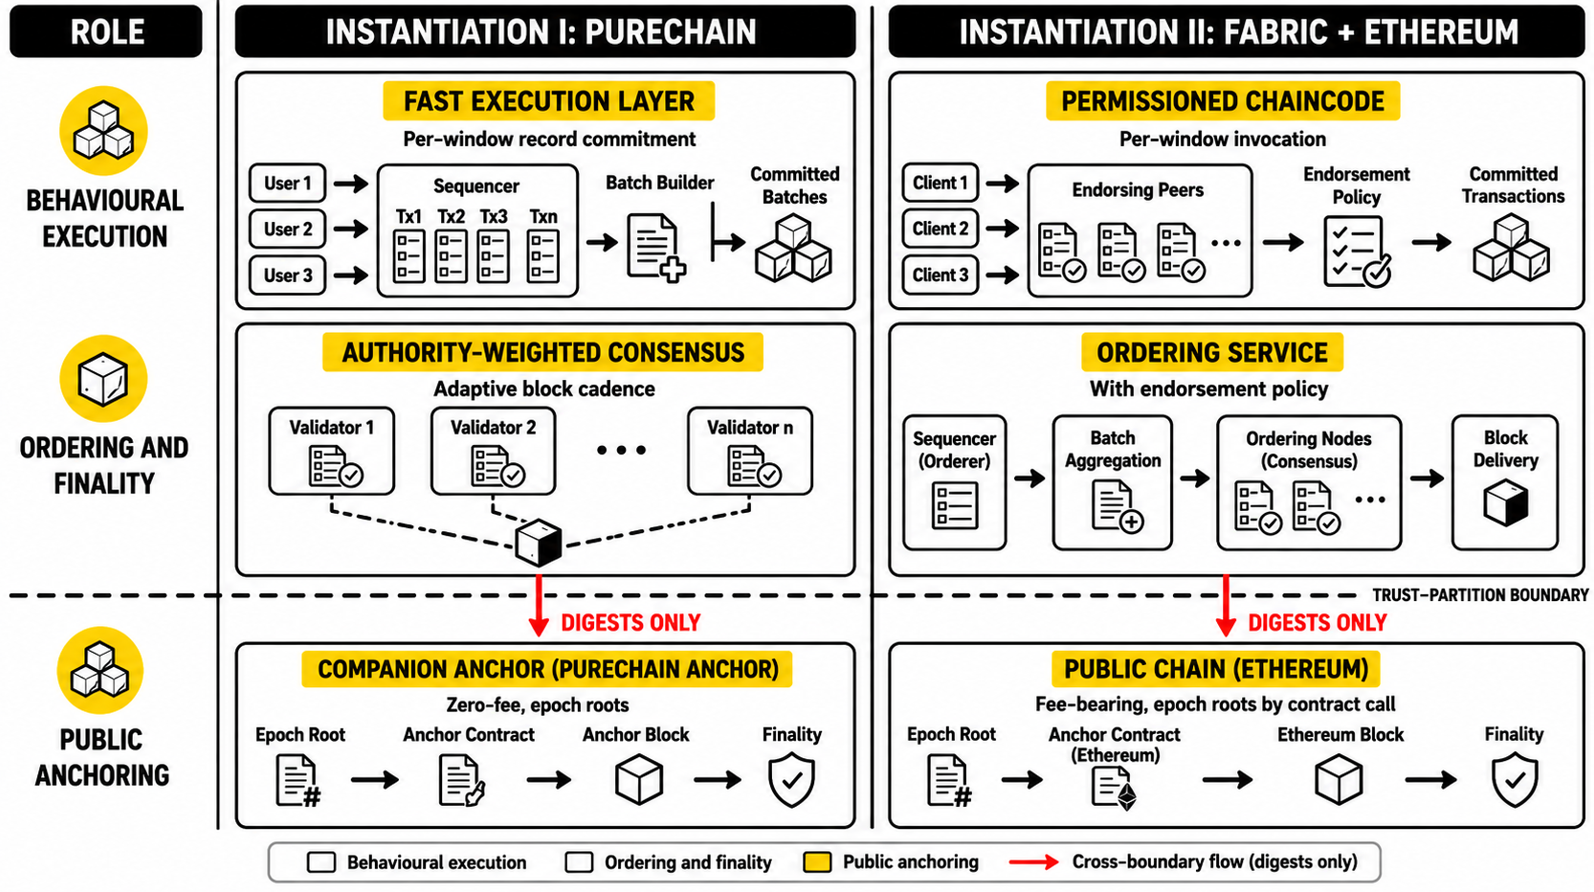
\includegraphics[width=1.00\textwidth]{figures/Picture21.PNG}
  \caption{The trust partition realised on PureChain NSL and on Fabric with Ethereum, with architectural roles held constant and the components discharging them substituted.}
  \label{fig:substrate-instantiation}
\end{figure}

\subsection{Experimental Environment}
\label{sec:substrate-environment}

Reproduction of either instantiation requires the substrate configuration, the class of device on which the constrained-side operations were executed, and the workload under which the measurements reported in the following chapter were taken. Tables~\ref{tab:env-instantiation-i} and~\ref{tab:env-instantiation-ii} record these in a common row order, so that a reader comparing them can see which quantities are substrate-dependent and which are not.

\begin{table}[tb]
  \centering
  \footnotesize
  \setlength{\tabcolsep}{5pt}
  \renewcommand{\arraystretch}{1.3}
  \caption{Experimental environment for Instantiation~I on PureChain NSL.}
  \label{tab:env-instantiation-i}
  \begin{tabularx}{\textwidth}{@{}
      >{\raggedright\arraybackslash}p{4.4cm}
      >{\raggedright\arraybackslash}X@{}}
    \toprule
    \textbf{Item} & \textbf{Configuration} \\
    \midrule
    Permissioned substrate & PureChain network \\
    Consensus mechanism & Authority-weighted consensus with adaptive block cadence \\
    Public anchor & PureChain public anchor, zero-fee; two public Ethereum networks used for comparison \\
    Smart-contract toolchain & Remix Ethereum IDE, Solidity compiler 0.8.10 \\
    Blockchain-side workload & One smart contract, four transaction types \\
    Network emulation & GNS3 \\
    Host operating system & Xubuntu, Xfce desktop \\
    Aggregator hardware & 251.4~GB RAM, 3.9~TB storage \\
    Constrained device profile & Client-side footprint of 0.17~MB model memory, 3.1~ms inference latency, 0.42~mJ per prediction, 167~kB update payload \\
    Learning framework & Flower 1.9.0, TensorFlow 2.9.0, Anaconda Navigator 2.6.1 \\
    Behavioural model & One-dimensional CNN-LSTM: 57 input units, 16 convolutional units with ReLU, softmax output over 8 classes \\
    Federation size & Five clients, aggregated on a single host \\
    Learning rates & 0.001 for client updates, 0.05 for global aggregation \\
    Datasets & CIC-Collections2023 public benchmark; and an internally generated lightweight IIoT dataset of 5{,}000 samples over 57 features, covering normal, denial-of-service, port-scan and brute-force traffic \\
    Training rounds & Twenty federated communication rounds \\
    \bottomrule
  \end{tabularx}
\end{table}

\begin{table}[tb]
  \centering
  \footnotesize
  \setlength{\tabcolsep}{5pt}
  \renewcommand{\arraystretch}{1.3}
  \caption{Experimental environment for Instantiation~II on Fabric with Ethereum.}
  \label{tab:env-instantiation-ii}
  \begin{tabularx}{\textwidth}{@{}
      >{\raggedright\arraybackslash}p{4.4cm}
      >{\raggedright\arraybackslash}X@{}}
    \toprule
    \textbf{Item} & \textbf{Configuration} \\
    \midrule
    Permissioned substrate & Hyperledger Fabric v2.5, Raft ordering \\
    Public substrate & Ethereum Geth v1.13, proof-of-work, 14~s mean block time, confirmation depth of three \\
    Topology & Five Fabric peers, one ordering service, one Geth node \\
    Block parameters & Two-second block interval, batch size of ten transactions \\
    Smart-contract toolchain & Remix IDE, Solidity compiler 0.8.17 \\
    Network emulation & Mininet v2.3.0, links at 10~Mbps and 1~Gbps \\
    Host operating system & Ubuntu 20.04.5 LTS \\
    Node hardware & Intel Xeon Gold 6230, 20 cores, 64~GB RAM, 2~TB SSD \\
    Constrained device class & Raspberry Pi 4, Cortex-A72, 4~GB RAM; ESP32 modules \\
    Edge workload & Lattice-encrypted payloads of 128 bytes at 10~Hz, signed and verified over five-minute steady-state runs \\
    Learning framework & TensorFlow 2.13, PennyLane 0.41.0, Anaconda Navigator 2.5.2 \\
    Behavioural model & CNN-LSTM trained centrally; no federation \\
    Dataset & NSL-KDD, 41 features, 5 classes, 80/20 stratified split \\
    Training configuration & Adam at learning rate 0.002, batch size 64, 15 epochs, ReLU activation, sparse categorical cross-entropy \\
    Transaction workload & 100 to 1000 simulated devices, 1000~tx/s on Fabric, cross-chain anchoring to Ethereum \\
    Repetition & Ten runs per measurement point, deviation below five per cent \\
    \bottomrule
  \end{tabularx}
\end{table}

The PureChain deployment is operated as a shared network rather than provisioned per experiment, so its validator membership and block cadence are fixed by the network operator and are not varied here. Identity and post-quantum operations were exercised on a separate bench rather than inside either ledger testbed, and Table~\ref{tab:env-identity} records that configuration. Keeping it distinct matters for interpretation: the encapsulation and compression measurements characterise the primitive on a workstation, not the cost of running it on the constrained devices listed above.

\begin{table}[tb]
  \centering
  \footnotesize
  \setlength{\tabcolsep}{5pt}
  \renewcommand{\arraystretch}{1.3}
  \caption{Environment for identity derivation and post-quantum key encapsulation.}
  \label{tab:env-identity}
  \begin{tabularx}{\textwidth}{@{}
      >{\raggedright\arraybackslash}p{4.4cm}
      >{\raggedright\arraybackslash}X@{}}
    \toprule
    \textbf{Item} & \textbf{Configuration} \\
    \midrule
    Host operating system & Windows 11 with WSL2, Ubuntu 24.04 LTS \\
    Hardware & Intel Core i7, 16~GB RAM \\
    Encapsulation mechanism & Kyber512, PQClean implementation \\
    Compression library & zlib v1.2.13 \\
    Implementation language & C, compiled with GCC \\
    Entropy seed length & 512 bits \\
    Ledger frameworks & Hyperledger Fabric for identity lifecycle; Ethereum on a Ganache testnet for revocation audit \\
    Scope of realisation & Identity derivation, compressed ciphertext delivery and reuse-aware decoding implemented; the ledger bridge specified but not implemented \\
    \bottomrule
  \end{tabularx}
\end{table}
The two environments differ in three respects that bear directly on how the following chapter should be read. Training is federated across five clients in the first instantiation and centralised in the second, so behavioural results are not directly comparable between them and are reported separately. The datasets likewise differ, the first instantiation evaluating on a public benchmark together with an internally generated IIoT set of 57 features and the second on NSL-KDD with 41 features across five classes. Anchoring economics differ by construction, the first instantiation writing to a zero-fee anchor and the second to a fee-bearing public chain with a fourteen-second block time and a confirmation depth of three.

What does carry across is the partition itself. Behavioural scoring is committed per observation window on a fast permissioned layer in both, finalisation is decided by a bounded identified validator set in both, and the material crossing to the public side is a digest in both. The measurements that follow are therefore reported per instantiation, and the cross-substrate claim rests on the structural correspondence. 
 